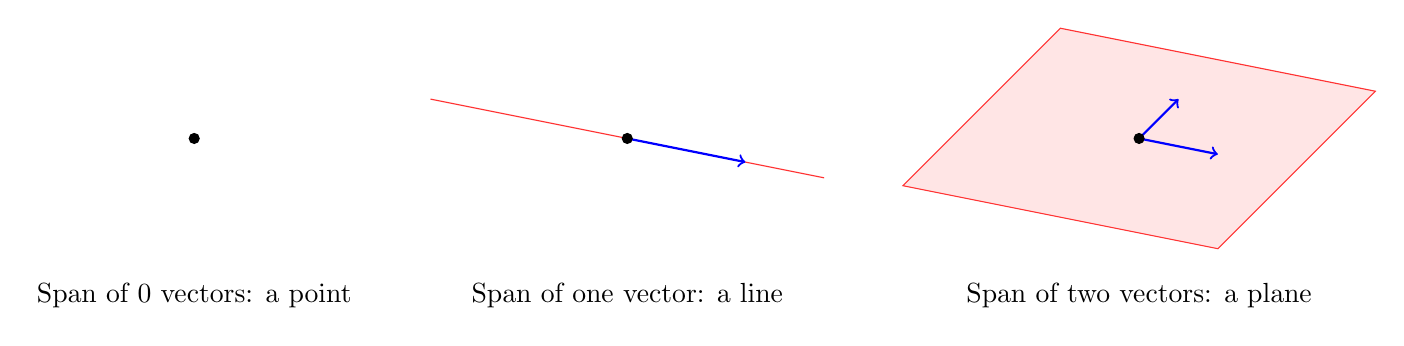
\begin{tikzpicture}
    \begin{scope}[xshift=-6cm]
      \draw[fill](0,0) circle [radius=1.8pt];
      \path(0,-2) node {Span of 0 vectors: a point};
    \end{scope}
    \begin{scope}[xshift=-0.5cm]
      \begin{scope}[x={(1cm,-0.2cm)},y={(0.5cm,0.5cm)}]
        \draw[red!80](-2.5,0) -- (2.5,0);
        \draw[->, thick, blue](0,0) -- +(1.5,0);
        \draw[fill](0,0) circle [radius=1.8pt];
      \end{scope}
      \path(0,-2) node {Span of one vector: a line};
    \end{scope}
    \begin{scope}[xshift=6cm]
      \begin{scope}[x={(1cm,-0.2cm)},y={(0.5cm,0.5cm)},z={(0cm,1cm)}]
        \filldraw[draw=red!80,fill=red!10](-2,-2,0) -- (2,-2,0) -- (2,2,0) -- (-2,2,0) -- cycle;
        \draw[->, thick, blue](0,0) -- +(0,1,0);
        \draw[->, thick, blue](0,0,0) -- +(1,0,0);
        \draw[fill](0,0) circle [radius=1.8pt];
      \end{scope}
      \path(0,-2) node {Span of two vectors: a plane};
    \end{scope}
  \end{tikzpicture}
